\section{Experiments}
\label{sec:experiments}

\begin{figure*}[t]
    \centering
    \subfigure[] {
        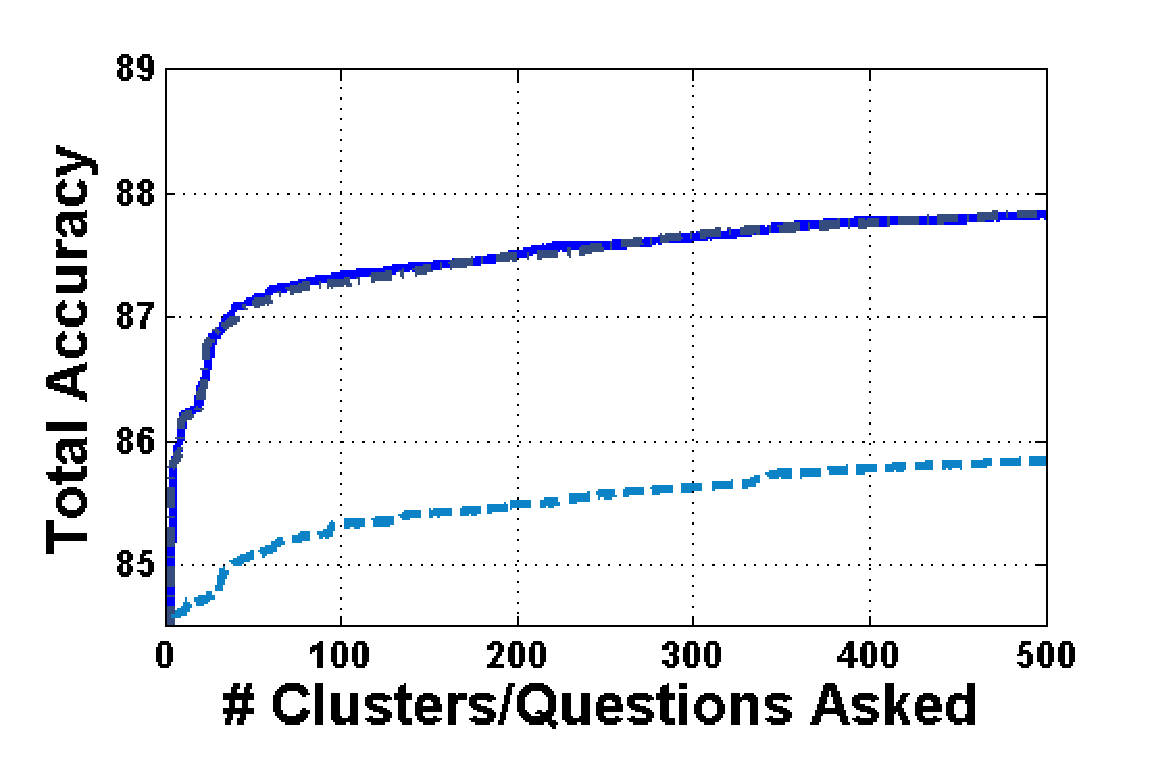
\includegraphics[width=0.31\textwidth]{dblp_seeding_compare.eps}
        \label{fig:first1}
    }
    \subfigure[] {
        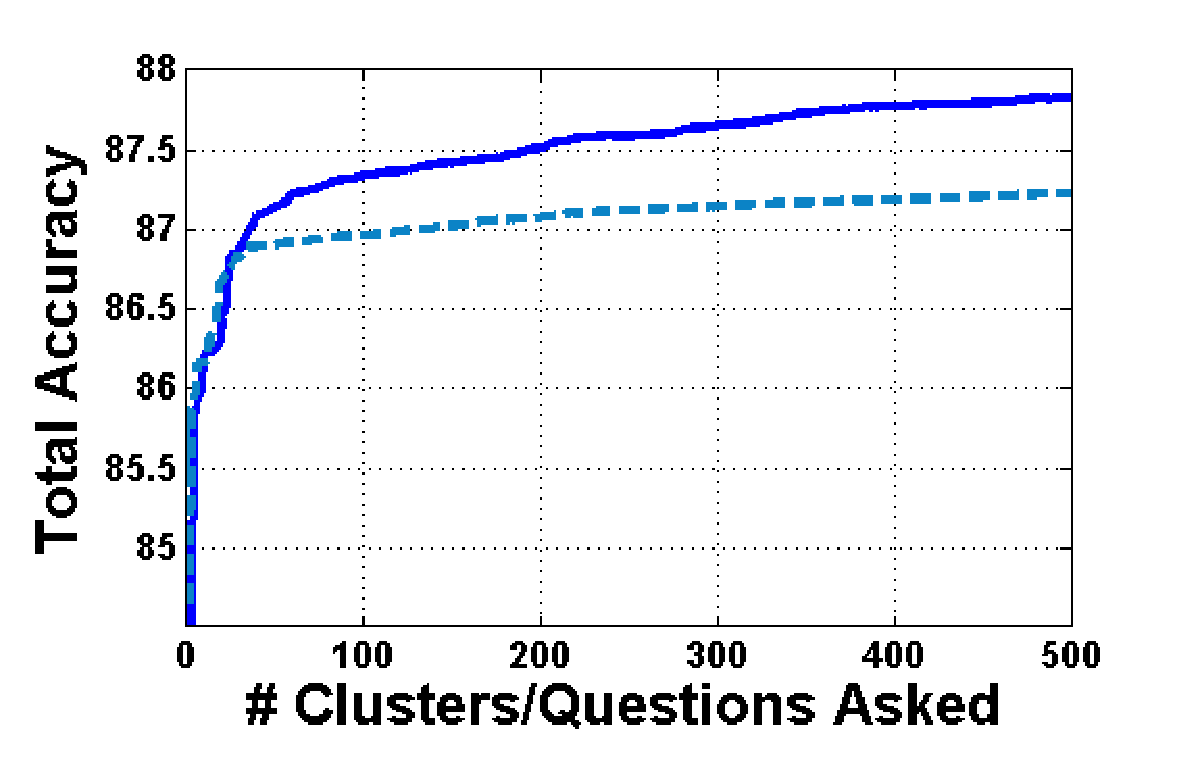
\includegraphics[width=0.31\textwidth]{dblp_clustering_compare.eps}
        \label{fig:first2}
    }
    \subfigure[] {
        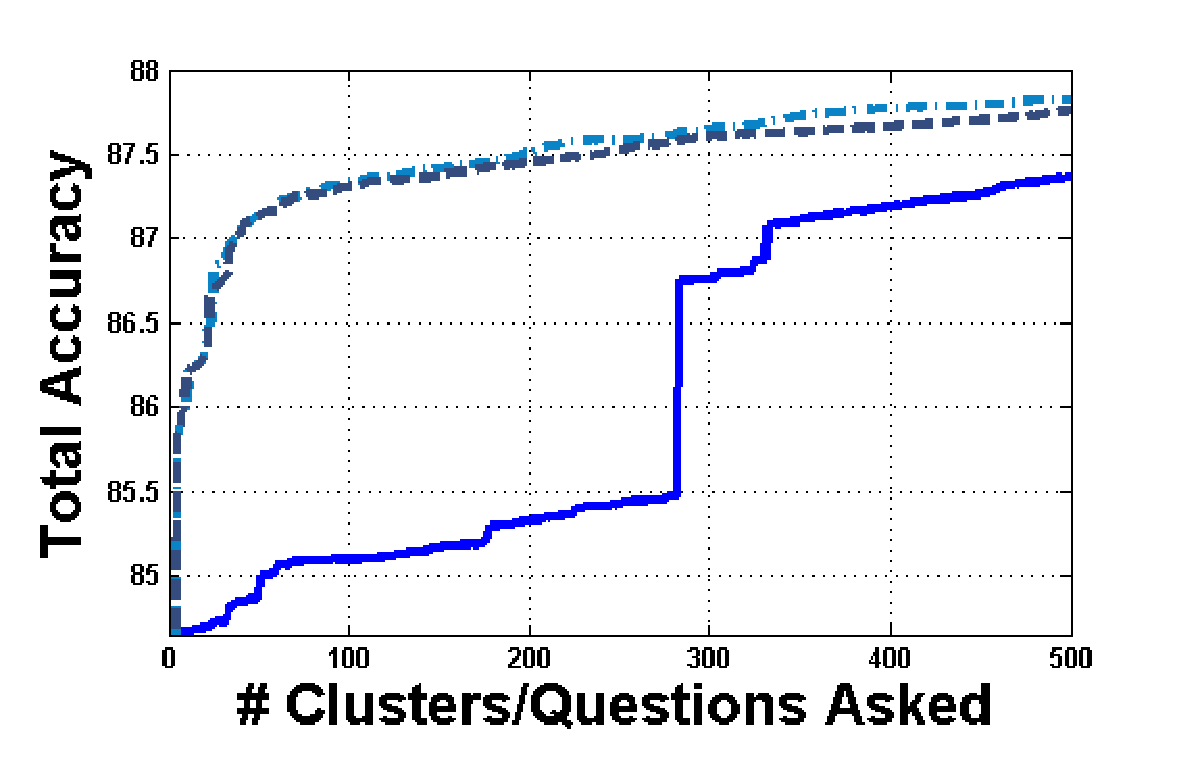
\includegraphics[width=0.31\textwidth]{dblp_ranking_compare.eps}
        \label{fig:first3}
    } \\
    \subfigure[] {
        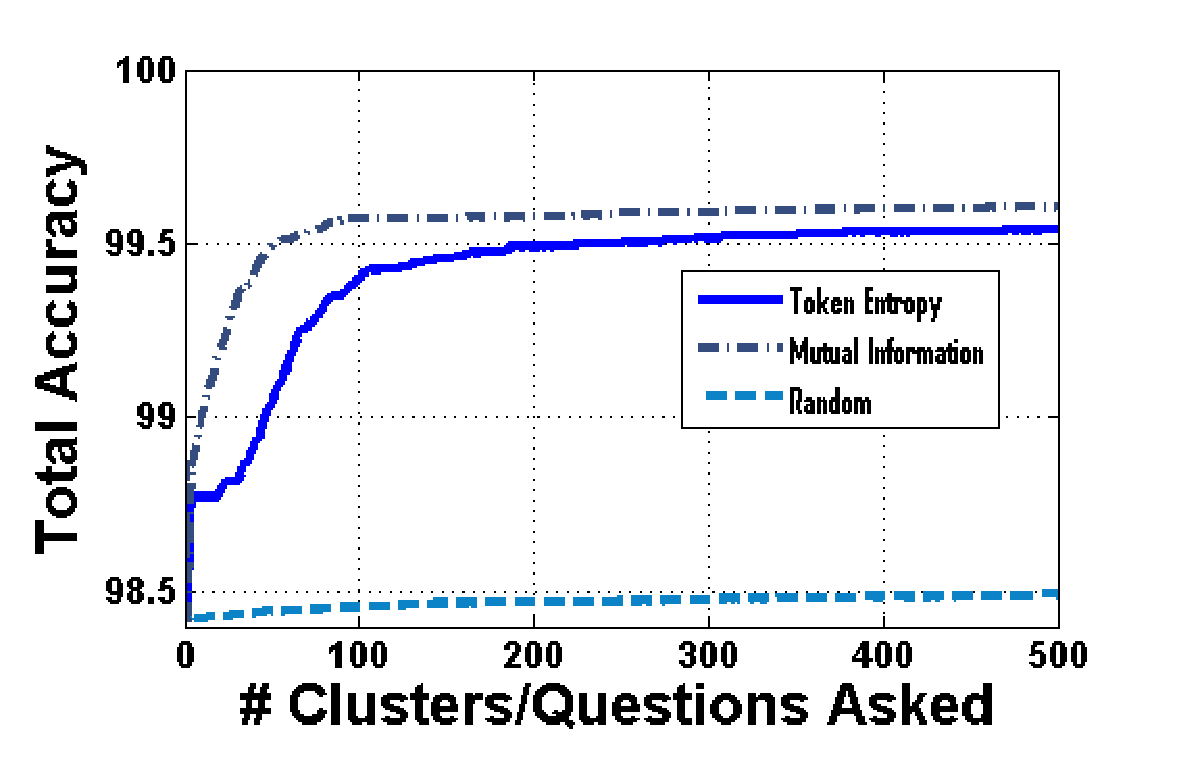
\includegraphics[width=0.31\textwidth]{pubmed_seeding_compare2.eps}
        \label{fig:first4}
    }
    \subfigure[] {
        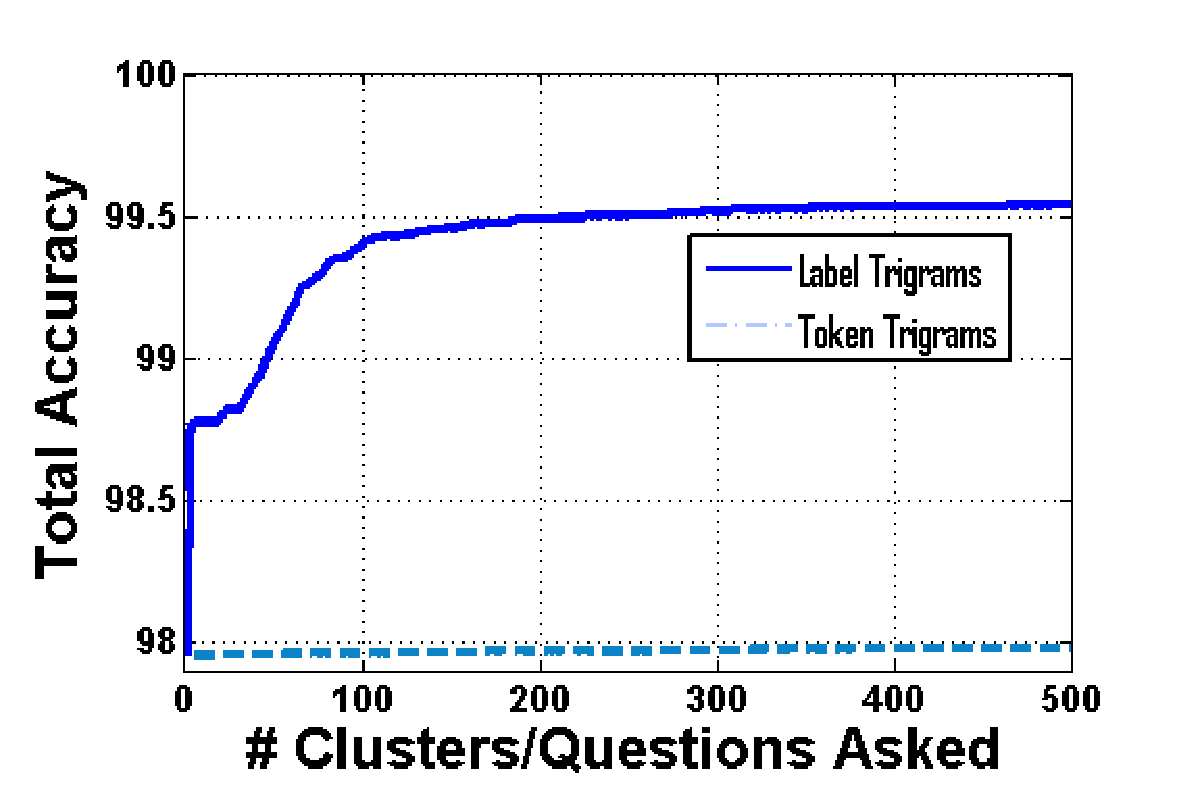
\includegraphics[width=0.31\textwidth]{pubmed_clustering_compare2.eps}
        \label{fig:first5}
    }
    \subfigure[] {
        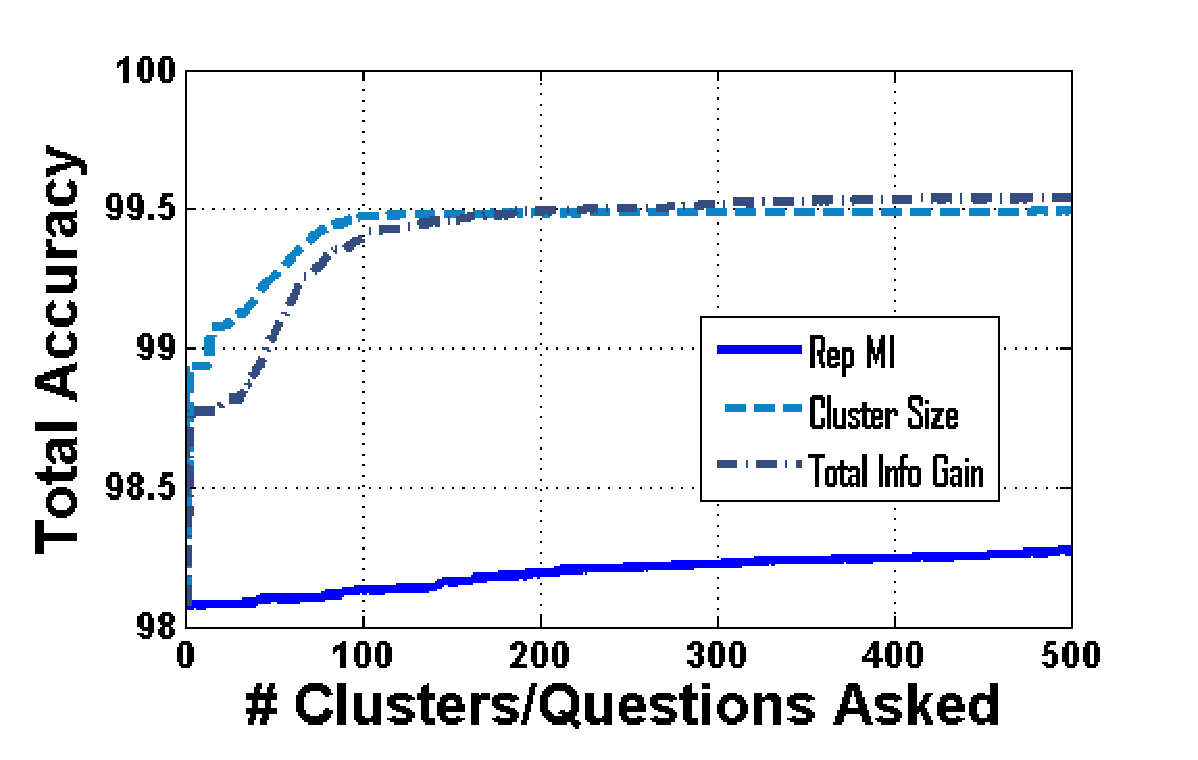
\includegraphics[width=0.31\textwidth]{pubmed_ranking_compare2.eps}
        \label{fig:first6}
    }
    \caption{Accuracy improvements for various selection parameters.  The first row is for the DBLP data set and the second is for PubMed.  From the left to right the columns compare the filtering, clustering, and ranking methods mentioned in this paper.  The parameter legend applies to both plots in each column.  Where not explicily being compared, the defaults are Mutual Information, Same Label, and Total Information Gain, respectively.}
    \label{fig:selectionExp}
\end{figure*}

In this section we demonstrate the effectiveness of our selection and integration approaches on sets of synthetic and real data.  

\subsection{Setup and Data Sets}
\label{sec:setup}

We extracted 14,000 labeled citations from the DBLP\footnotemark\footnotetext[1]{http://kdl.cs.umass.edu/data/dblp/dblp-info.html} and 500,000 from the PubMed\footnotemark\footnotetext[2]{http://www.nlm.nih.gov/bsd/licensee/medpmmenu.html} databases.  For unlabeled testing data, we removed the labels and concatenated text from each of the available fields.  Order of fields was randomly mixed in keeping with real-life inconsistency of citation structure.

To test our selection methods without the effects of integration accuracy, we supplemented the ground truth values in place of Turker answers when running constrained inference, equivalent to a workforce of perfect Turkers.  To evaluate the integration techniques, we experimented with simulated answers as well as real answers from AMT.  For answer simulation we sampled the accuracy $Q_{i}$ of Turker $i$ from a normal distribution $\mathcal{N}(\mu,~\sigma)$ whose parameters we allowed to vary.  Where not listed explicitly, we used the values $\mu=0.5$ and $\sigma=0.3$.  We sampled the ground truth value with probability $Q_{i}$ and with probability $1-Q_{i}$ a random guess was used instead.

We also performed a set of experiments on Amazon Mechanical Turk using both datasets while varying question difficulty.  Each HIT consisted of 10 bibliographic token annotation tasks at \$0.10 per HIT, or \$0.01 per token. From the DBLP set we produced a set of 500 HITs and required users to pass a qualification test before being allowed to answer questions.  We produced an additional ``hard" set where the same questions were stripped of any punctuation and no qualification test was used.  The motivation was to develop questions of a more ambiguous nature likely to cause more conflicts.  We coined this set DBLP-hard.  The PubMed set consisted of 500 questions and also required no such qualification test.  Some of the more ambiguous questions were selected to further test confusion among Turkers and study conflict.  In all sets 5 Turkers were assigned to each HIT and quality was assessed on a per HIT basis using the Dawid \& Skene method.

\subsection{Selection Experiments}

%\begin{figure}
    %\centering
    %\subfigure[DBLP] {
        %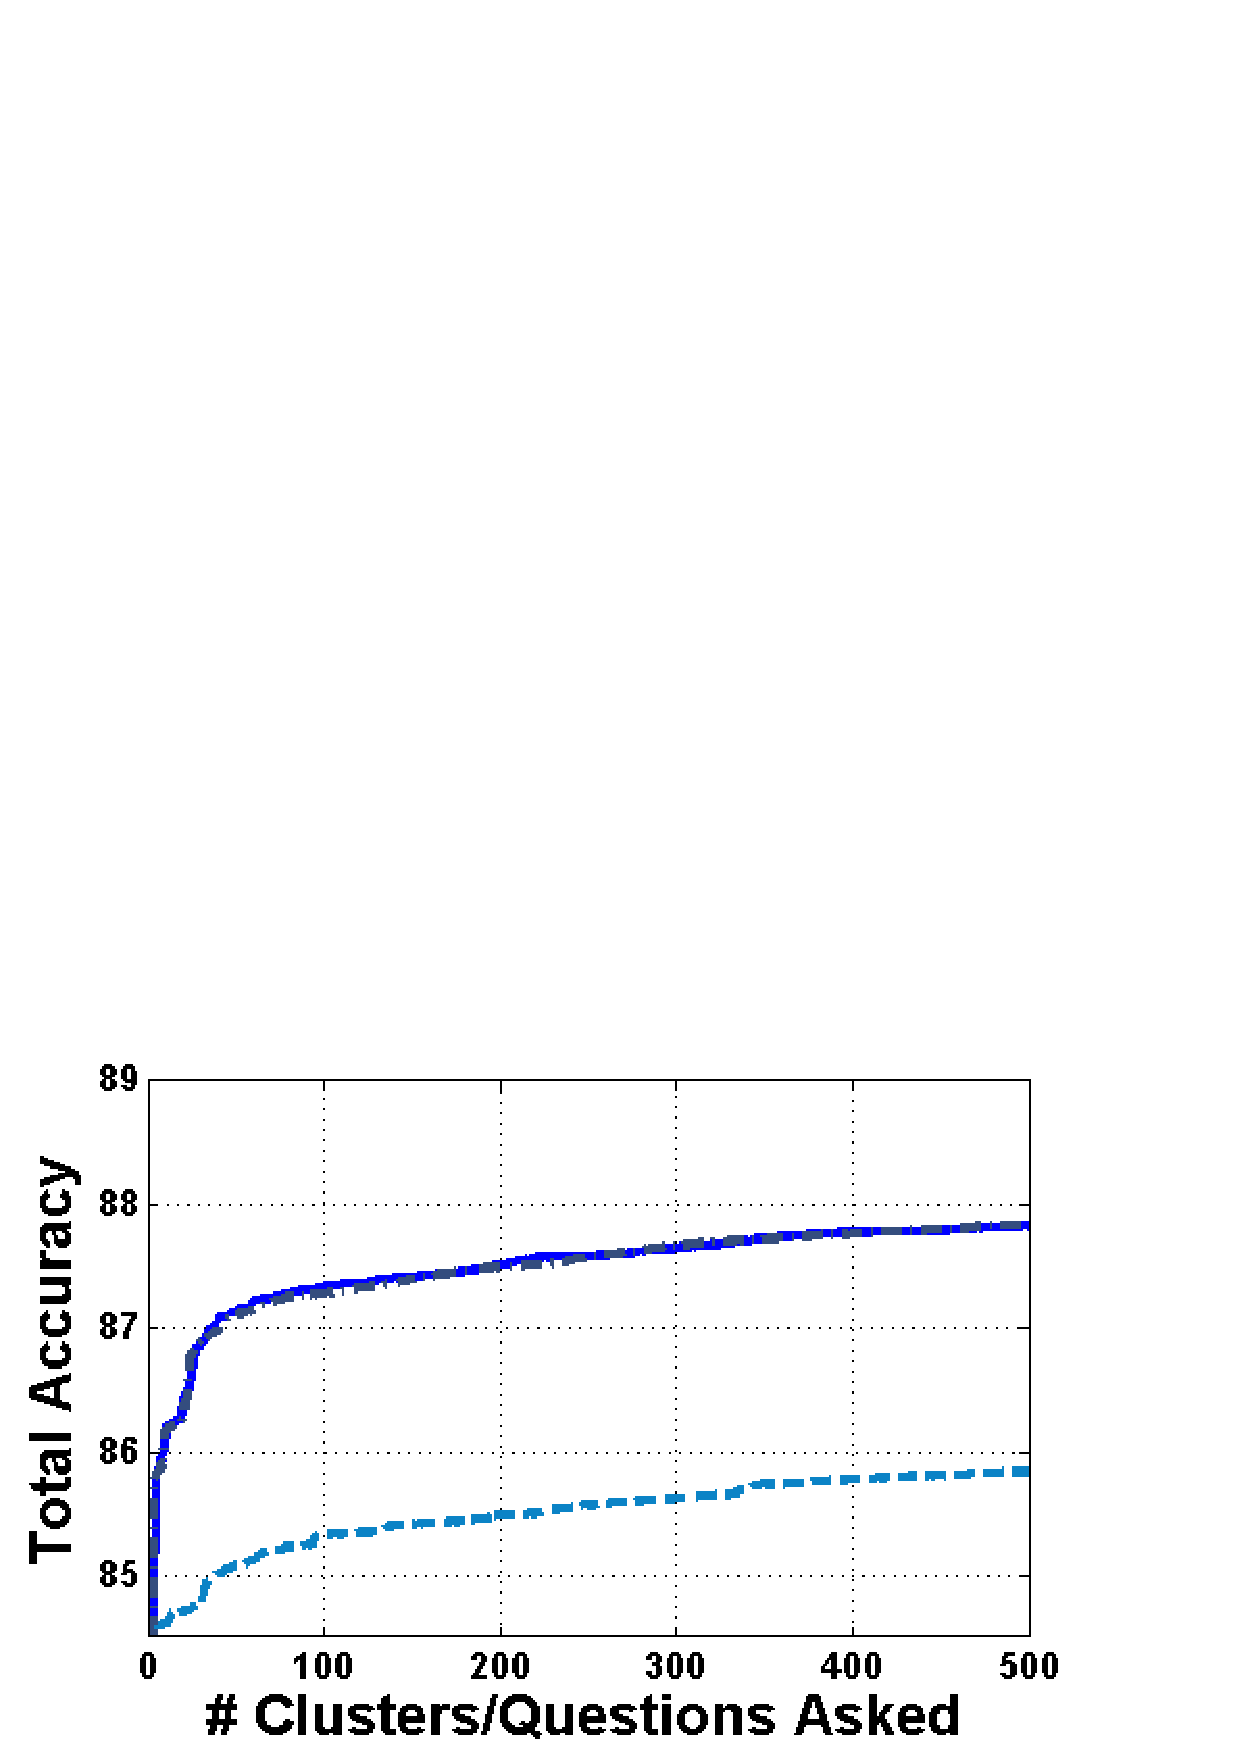
\includegraphics[width=0.22\textwidth]{images/dblp_seeding_compare.png}
        %\label{fig:first1}
    %}
    %\subfigure[PubMed] {
        %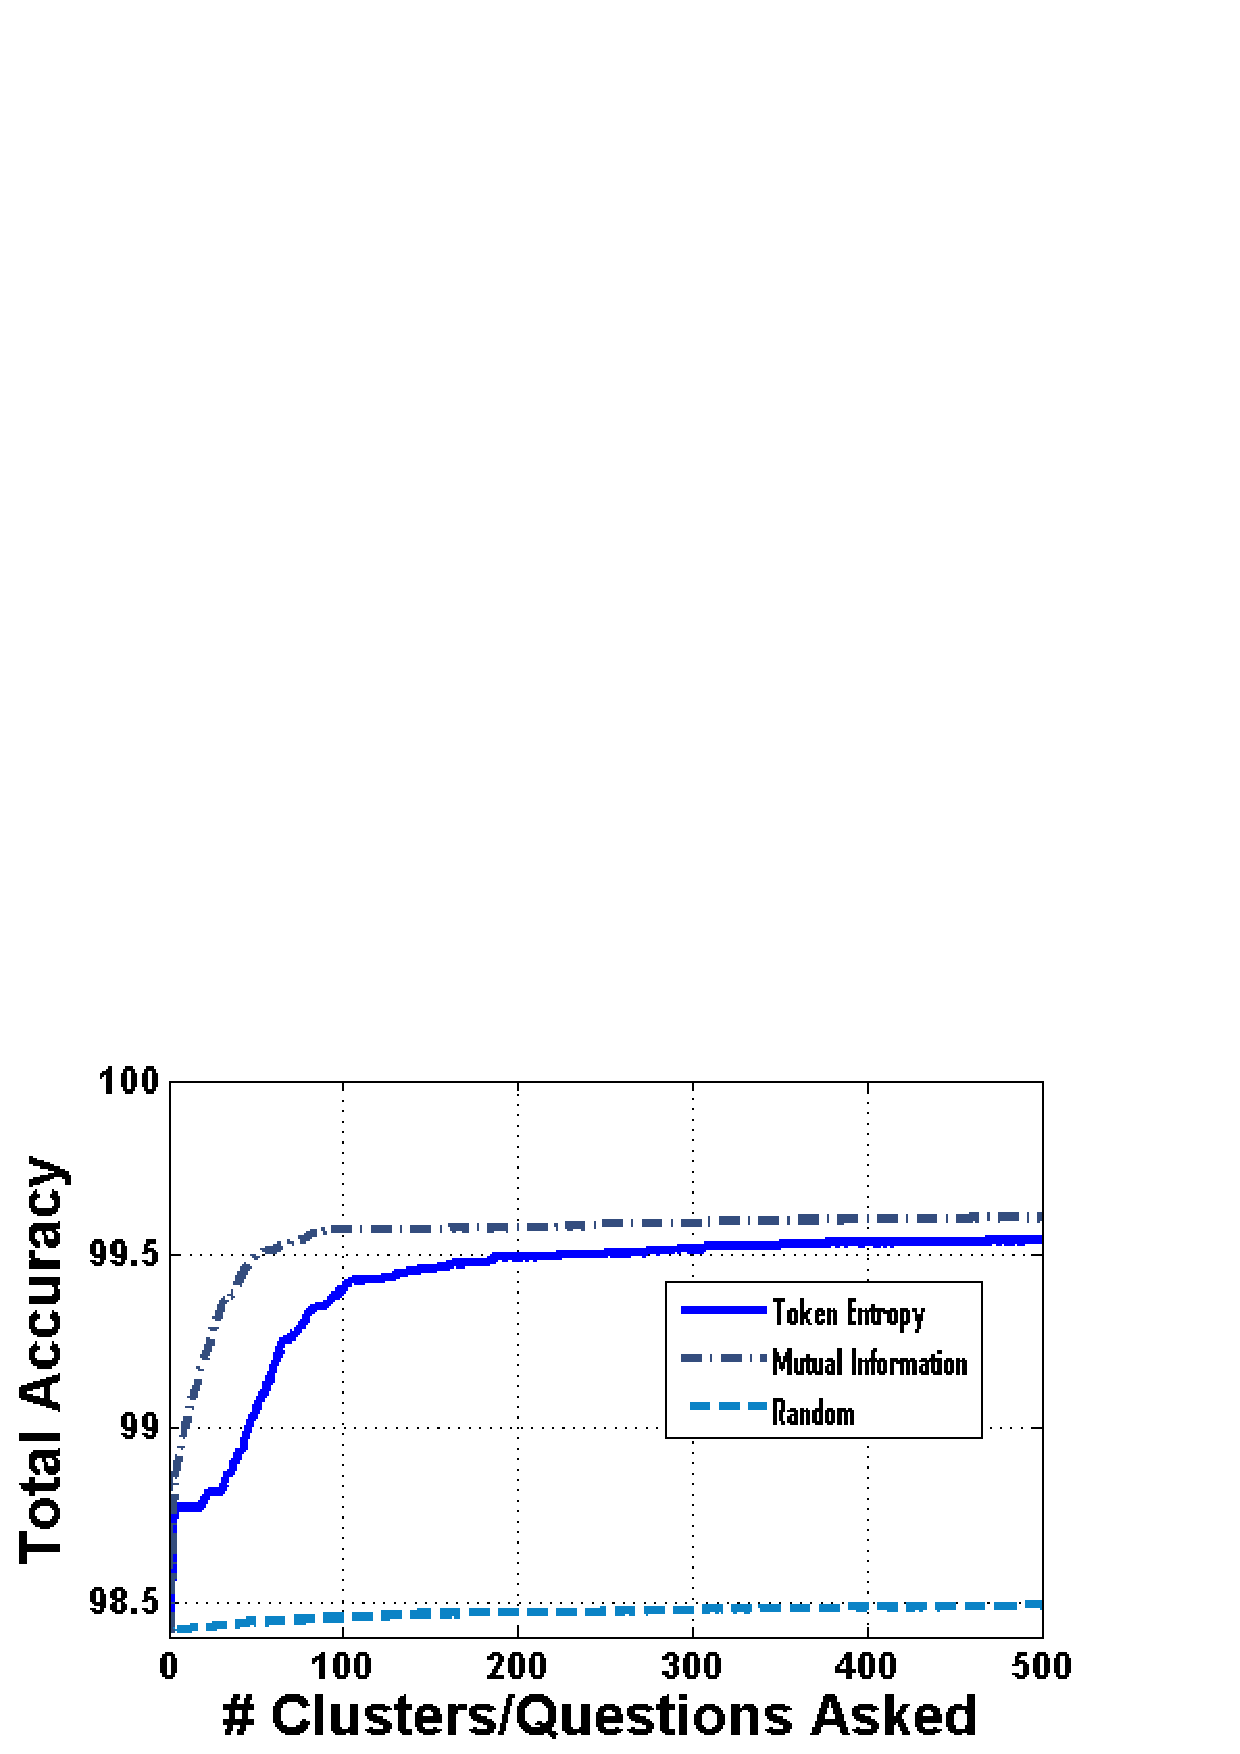
\includegraphics[width=0.22\textwidth]{images/pubmed_seeding_compare2.png}
        %\label{fig:second1}
    %}
    %\caption{Seeding comparison for (a) DBLP and (b) PubMed.  Default clustering is Same Label and default ranking is Total Entropy.}
    %\label{fig:select1}
%\end{figure}

Figures~\ref{fig:first1}-\ref{fig:first6} contain experiments comparing our various selection algorithms by detailing the accuracy improvements after a specific number of questions have been asked.  Tokens were selected based on the pipeline of Algorithm~\ref{alg:QuestionSelect} using a specific combination of filtering, clustering, and ranking approaches.  The choices for filtering were random selection, highest token entropy, and highest mutual information.  Clustering compares the token trigram and label trigram methods.  Finally, ranking looks at ordering by highest representative token mutual information, cluster size, and total information gain.  Where not explicitly listed, the default values were highest mutual information, label trigram, and total information gain, respectively.

To eliminate the possible variability of crowd answers and study purely the ability of the selection algorithms to identify highly inaccurate and highly impactful tokens, we supplied the ground truth as the answer after selection.  The cluster representative's answer (label) to each question (token) is applied to all subsequent tokens in its cluster.  A constrained Viterbi inference algorithm runs over all documents that are supersets of tokens belonging to question clusters.  The accuracy value in each figure represents the final token accuracy after running constrained inference.

%\begin{figure}
    %\centering
    %\subfigure[DBLP] {
        %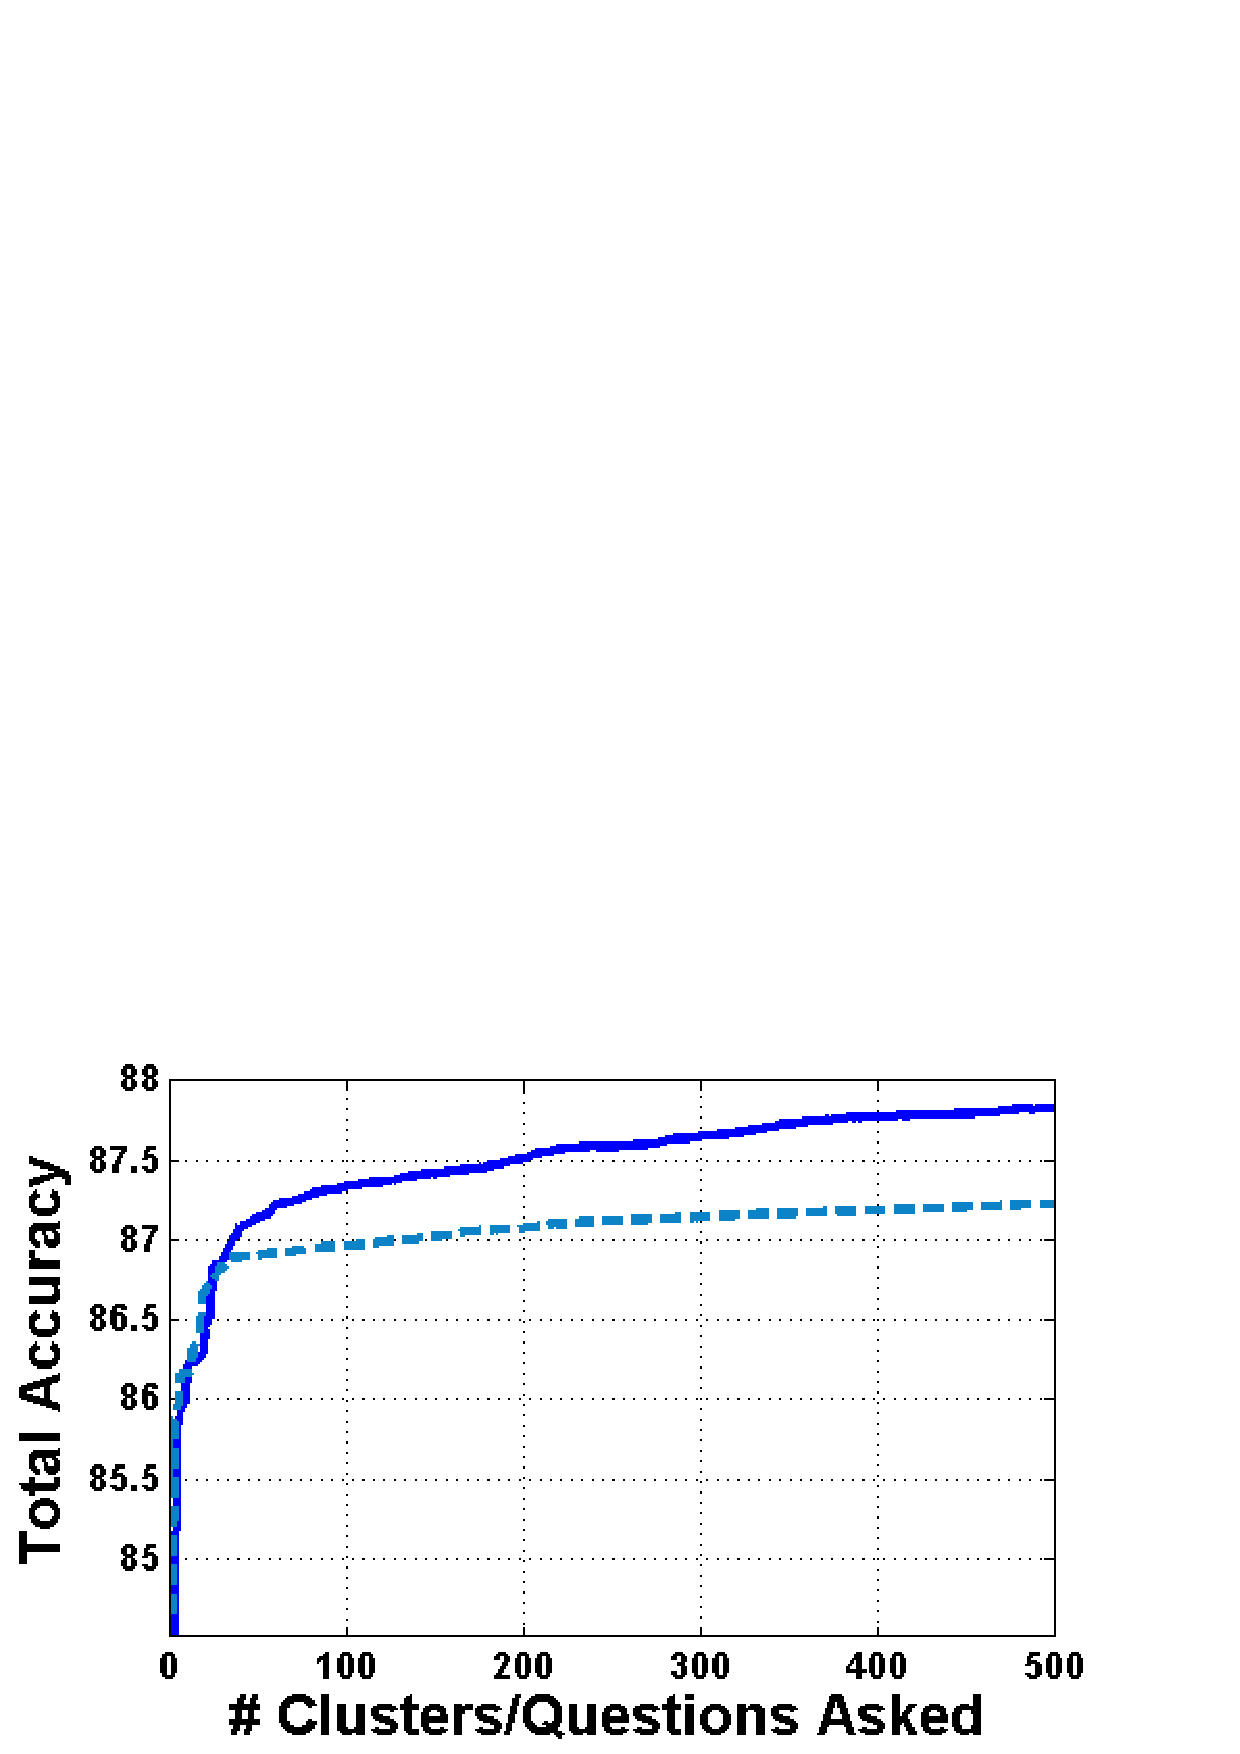
\includegraphics[width=0.22\textwidth]{images/dblp_clustering_compare.png}
        %\label{fig:first2}
    %}
    %\subfigure[PubMed] {
        %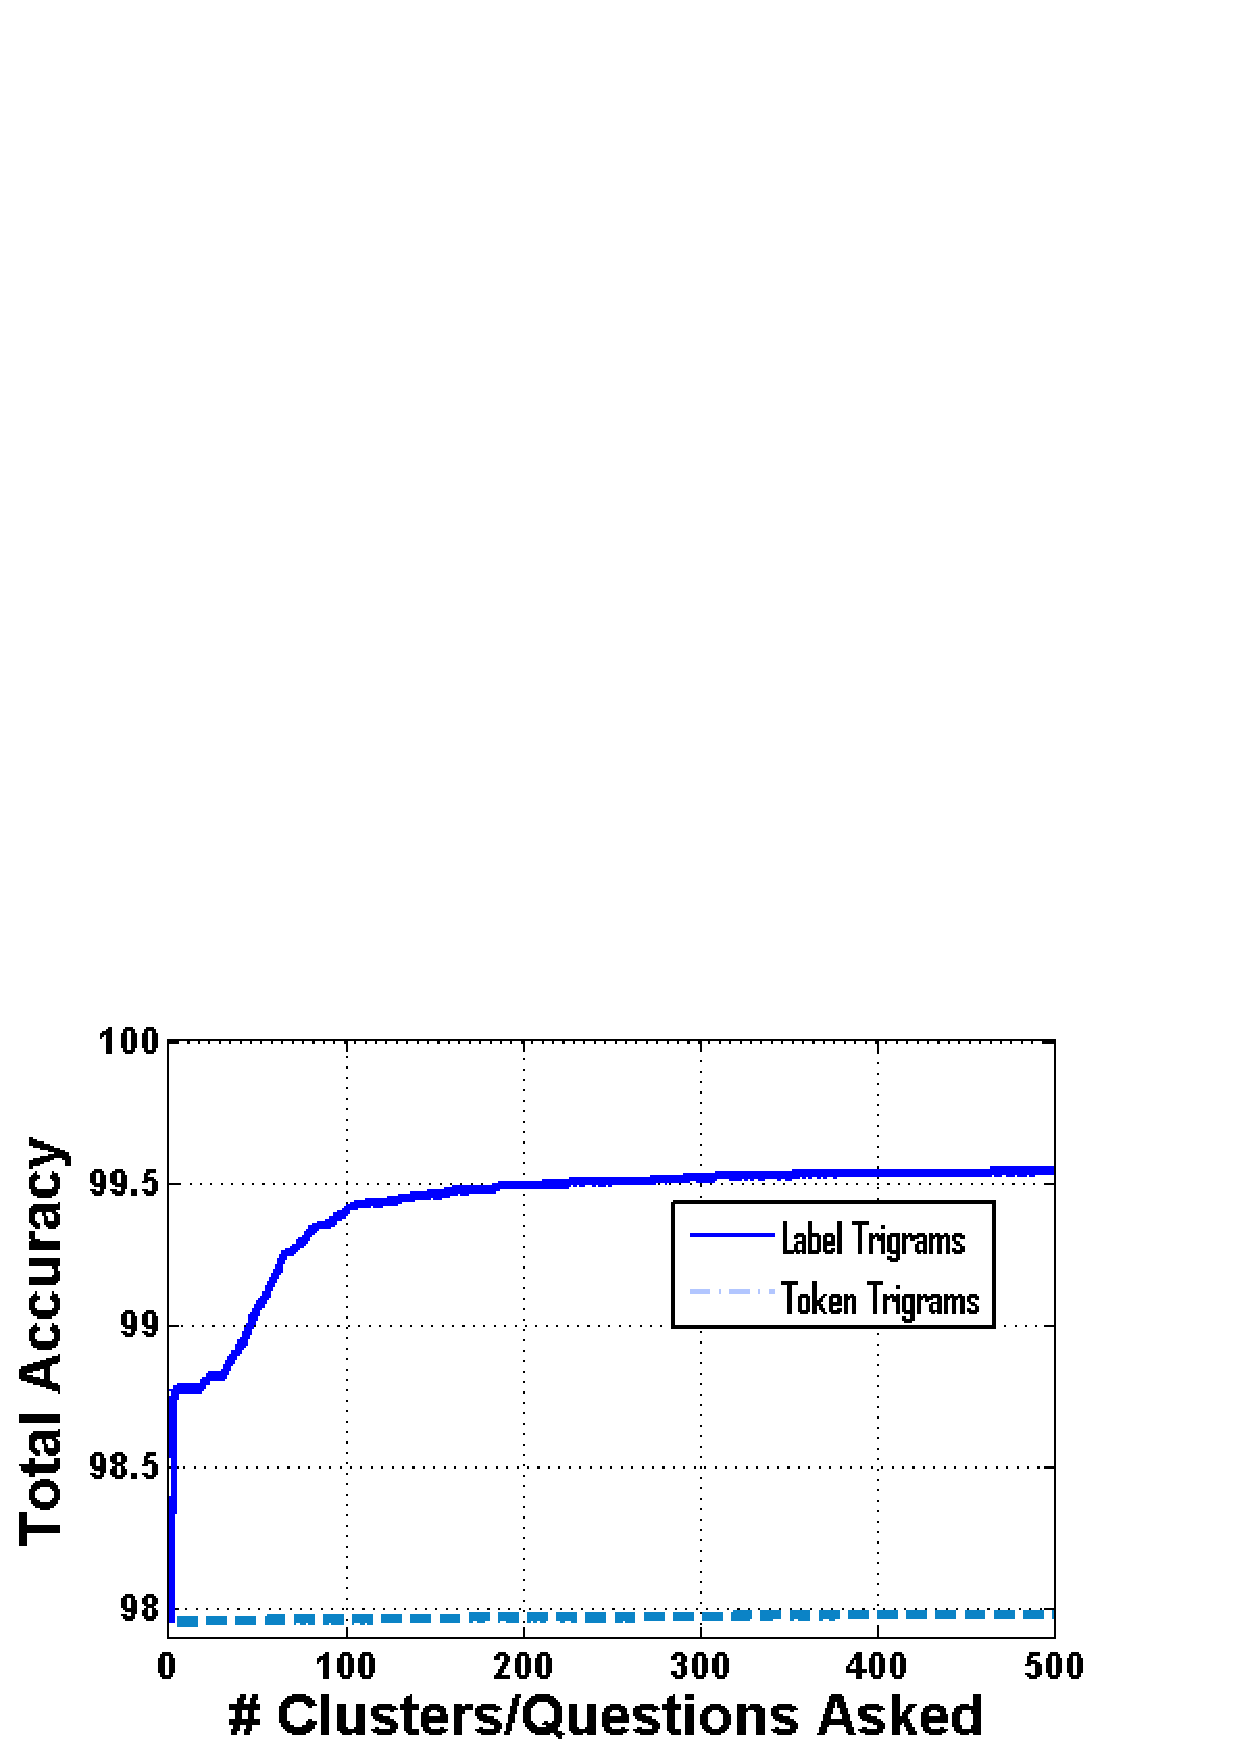
\includegraphics[width=0.22\textwidth]{images/pubmed_clustering_compare2.png}
        %\label{fig:second2}
    %}
    %\caption{Clustering comparison for (a) DBLP and (b) PubMed.  Default seeding is High Entropy and default ranking is Total Entropy.}
    %\label{fig:select2}
%\end{figure}

%In this paper, we proposed two possible functions for selecting a token from each document that maximized information gain.  High Entropy chooses that which has the highest marginal entropy over its labels while Neighborhood Entropy selects the token in the center of the largest 3-window pocket of marginal entropies.  Figures~\ref{fig:first1} \&~\ref{fig:first4} show the effectiveness of both methods when compared to randomly selecting a token.  While comparable in the DBLP set (\ref{fig:first1}), the PubMed set (\ref{fig:first4}) benefits greatly from extracting tokens with the highest Neighborhood Entropy.  Both methods reach accuracy values unobtainable by random selection in fewer than 10 questions.

The results of Figures~\ref{fig:first1} and~\ref{fig:first4} show a marked increase in accuracy using information theoretic techniques after just a few questions compared to selecting at random.  After about 25 questions in the DBLP set, both information theoretic methods produce a 5-fold increase in accuracy compared to random and reduce the overall error by about 15\%.  The initial PubMed accuracy was much better, but still saw a 66\% reduction in error using our selection methods after about 50 questions.  This is significant when considering DBLP contained 36k individual tokens and PubMed 3.3m tokens.  Each question only queries for the label to a single token, so we are seeing large reductions in error querying on significantly small fractions of the data. 

The trigram methods are compared in Figures~\ref{fig:first2} and~\ref{fig:first5}, where label trigrams outperform token trigrams in both data sets.  The knee in the PubMed set is due to several large clusters of similar tokens being selected first.  There are more likely to be misclassification errors using label trigrams, but experiments show the increased coverage outweighs this concern.  Finally, ranking metrics are compared in Figures~\ref{fig:first3} and~\ref{fig:first6}.  The presence of large clustering gives added weight to both methods that take cluster size into account.  Information gain, the sum of a mutual information scores of all tokens in a cluster, takes into account both cluster size and informativeness and excels in both data sets.

%Figures~\ref{fig:first2} \&~\ref{fig:first5} compare the possible clustering algorithms.  For the DBLP set (\ref{fig:first2}), there were zero clustering errors for Same Token and Same Field, and approximately 2\% of citations were clustered incorrectly using the Same Label approach.  The PubMed set (\ref{fig:first5}) also contained no errors for the constrictive Same Token and Same Field, but approximately a 0.2\% error rate for Same Label. Despite introducing additional errors, the gain from clustering a larger number of tokens gives the Same Label mechanism a boost in overall token accuracy.  The gain is most drastic for the PubMed set, where the clusters were much larger.  Same Token and Same Field exhibited minimal clustering as evidenced by the nearly flat lines.

%The final set of selection experiments is shown in Figures~\ref{fig:first3} \&~\ref{fig:first6}.  There is very little difference between the Cluster Size and Total Entropy methods, but both easily eclipse ranking by the representative Highest Token Entropy and reach the same accuracy in 90\% fewer questions for DBLP.  PubMed results are similar, but orders-of-magnitude greater.

%One important comment is that these accuracies are truncated at 500 questions and given a large enough budget one could theoretically reach near-perfect accuracy.


%\begin{figure}
    %\centering
    %\subfigure[DBLP] {
        %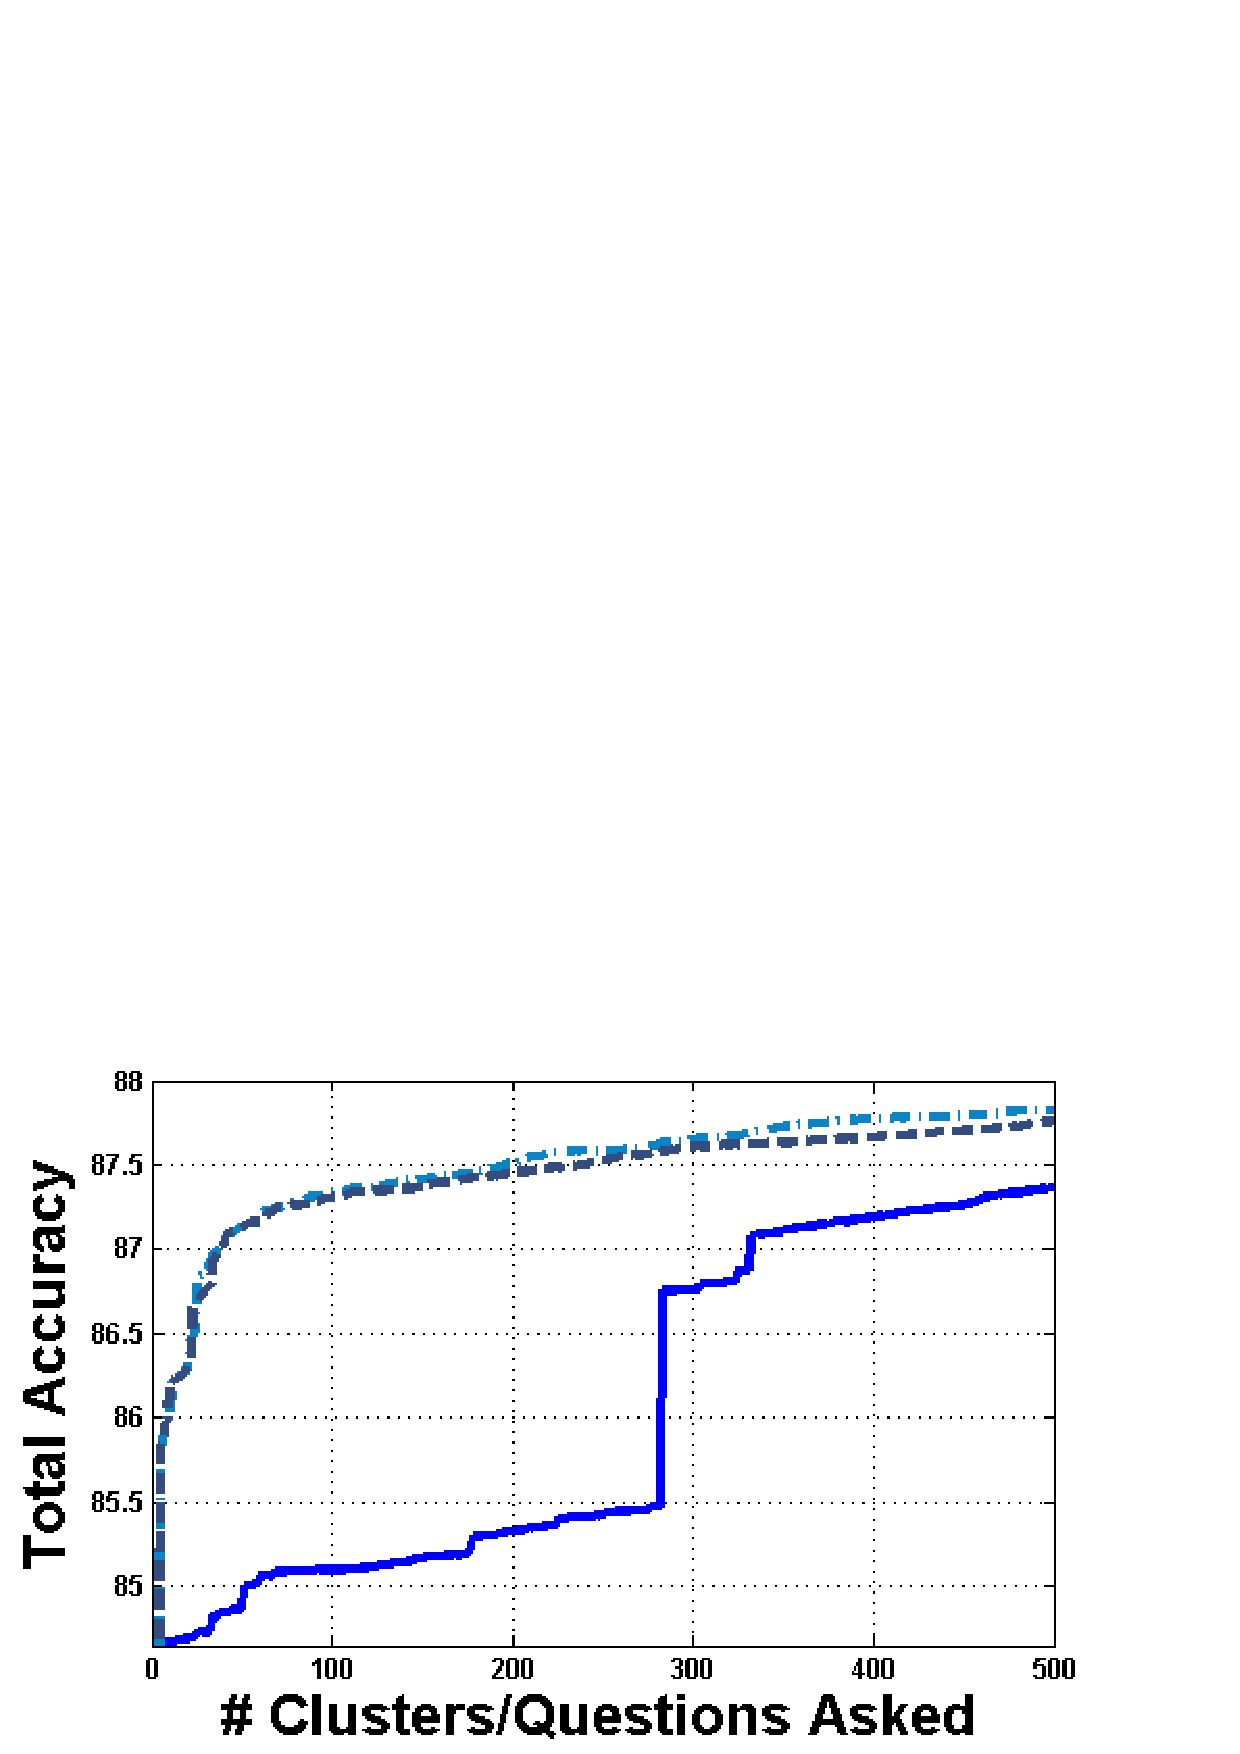
\includegraphics[width=0.22\textwidth]{images/dblp_ranking_compare.png}
    %}
    %\subfigure[PubMed] {
        %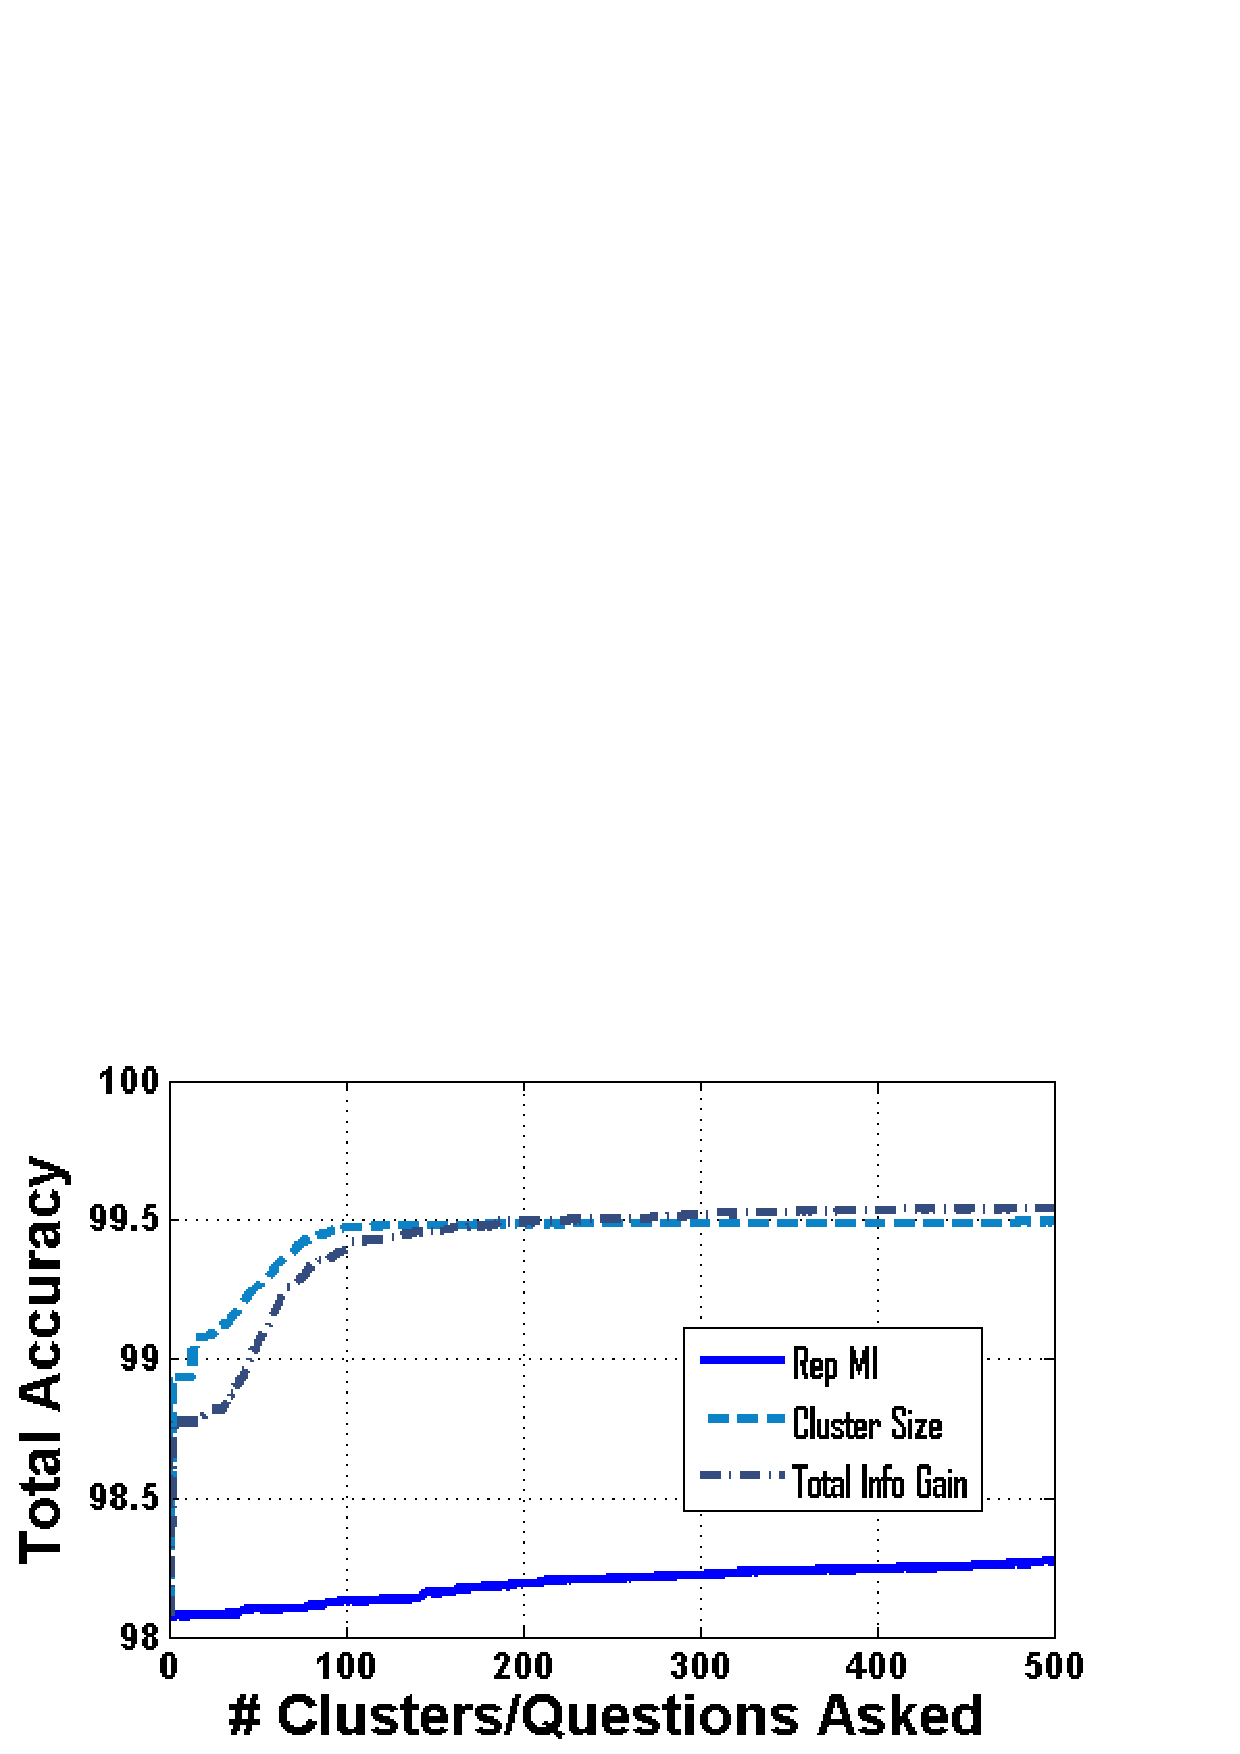
\includegraphics[width=0.22\textwidth]{images/pubmed_ranking_compare2.png}
    %}
    %\caption{Ranking comparison for (a) DBLP and (b) PubMed.  Default seeding is High Entropy and default clustering is Same Label.}
    %\label{fig:select3}
%\end{figure}

\subsection{Integration Experiments}
\begin{figure}[t]
	\centering
	\subfigure[]{        
	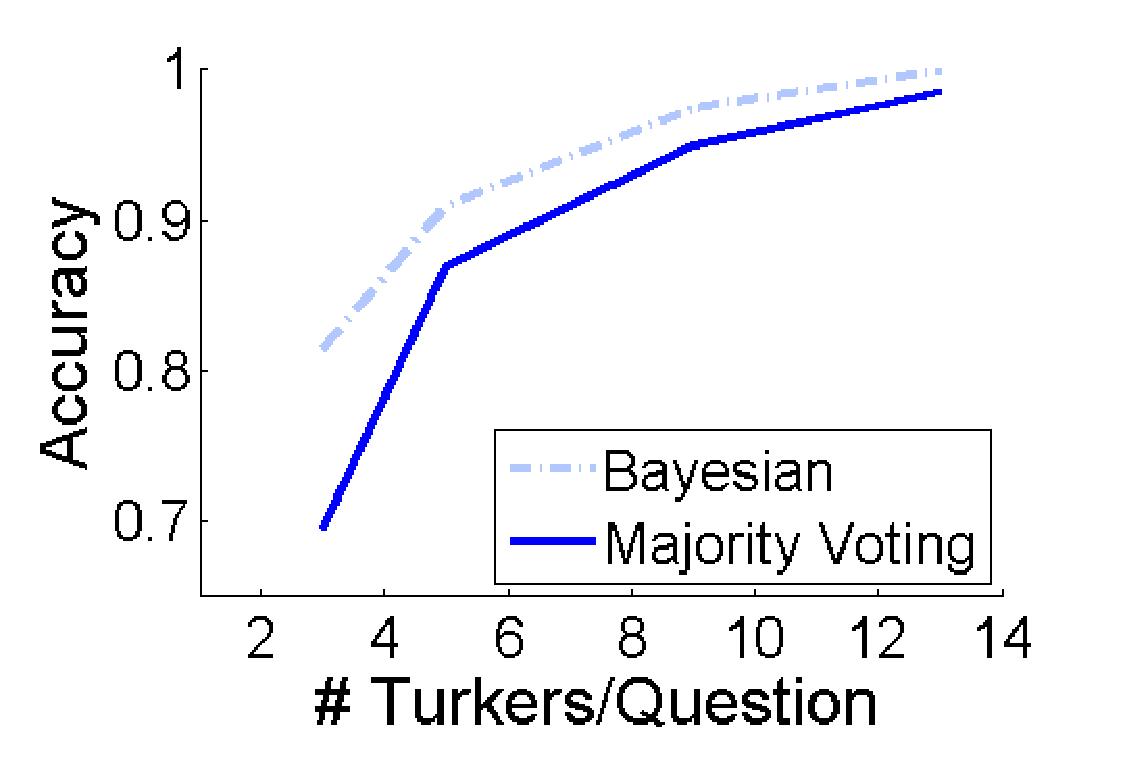
\includegraphics[width=0.47\textwidth]{integration_exp1_numT.eps}
        %\caption{Comparison of integration methods vs. number of Turkers per question for a synthetic set of 500 questions and Turker accuracies drawn from a mean of $0.5$ and standard deviation of $0.3$.}
        \label{fig:integrate1}
	}
\hspace{-4mm}
%\end{figure}
%\begin{figure}[t]
	\subfigure[]{
        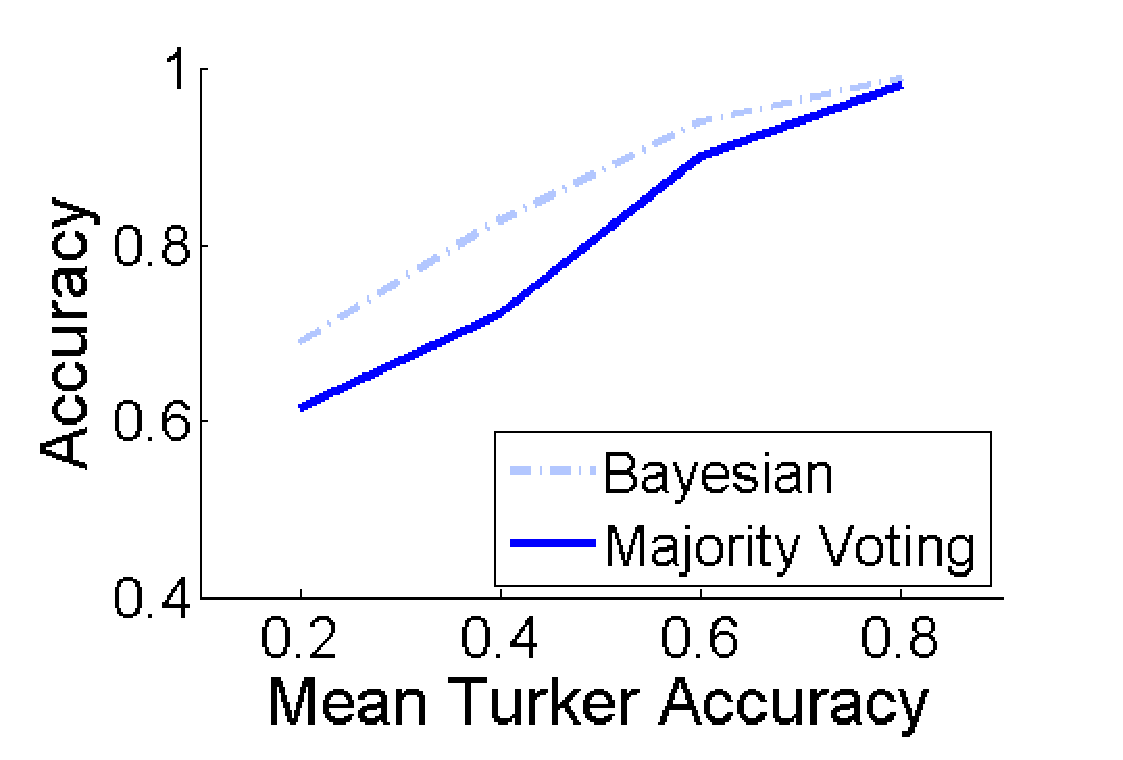
\includegraphics[width=0.47\textwidth]{integration_exp2_meanQ.eps}
        %\caption{Comparison of integration methods vs. average Turker quality for a synthetic set of 500 questions and 5 Turkers per question.}
        \label{fig:integrate2}
	}
	\caption{Comparison of integration methods versus (a) number of Turkers per question and (b) average Turker quality for a synthetic set of 500 questions.  Where not stated the default number of Turkers was 5 and mean accuracy was 0.5.}
%\vspace{-1mm}
\end{figure}

To measure the efficacy of our integration methods, we conducted experiments over both real and synthetically generated data.  The parameters of the synthetic model were listed in Section~\ref{sec:setup} and allowed us to vary both the number of Turkers answering questions and their individual quality values.

\eat{
%Answers received from the crowd have many variables that must be factored into a rigorous justification of any method of combination.  Primarily, we are concerned with measuring how the final combined accuracy is affected both by the number of redundant answers and by the actual quality of the workers.  A set of synthetic responses to real questions were generated in a manner that the allowed the average worker quality to be varied throughout the experiments.
}

\begin{figure}[t]
\subfigure[DBLP] {
    \centering
    \hspace{2.5cm}
%\begin{center}
    \scalebox{1.0}{
    \begin{tabular}{ | l | l |}
    \hline
    Integration Method & Accuracy \\ \hline
    Majority Vote & 97.5 \\ \hline
    Bayesian & 97.5 \\ \hline
    \end{tabular}
    }
\hspace{2.5cm}
%\end{center}
}\\
\subfigure[DBLP-hard] {
%\begin{center}
    \centering
    \hspace{2.5cm}
    \scalebox{1.0}{
    \begin{tabular}{ | l | l |}
    \hline
    Integration Method & Accuracy \\ \hline
    Majority Vote & 75.8 \\ \hline
    Bayesian & 77.3 \\ \hline
    \end{tabular}
    }
\hspace{2.5cm}
%\end{center}
}\\

\subfigure[PubMed] {
%\begin{center}
    \centering
    \hspace{2.5cm}
    \scalebox{1.0}{
    \begin{tabular}{ | l | l |}
    \hline
    Integration Method & Accuracy \\ \hline
    Majority Vote & 14.3 \\ \hline
    Bayesian & 20.9 \\ \hline
    \end{tabular}
    }
    \hspace{2.5cm}
%\end{center}
}
\caption{Amazon Mechanical Turk accuracies for a set of 500 standard (DBLP) and two sets of 500 difficult (DBLP-hard \& PubMed) questions.}
\label{fig:table}
\end{figure}

\eat{
%Workers were automatically generated by selecting a quality value $Q \in [0,1]$ from a Gaussian distribution of standard deviation 0.3 and a mean that varies over the experiment.  Quality values drawn outside the $[0,1]$ range were truncated at the boundary.  Each worker was assigned to a 'HIT', which constituted a set of 10 questions.  The quality level dictated the generation of answers.  In keeping with our assumption of quality, the true label was applied with probability $Q$.  With probability $1-Q$, the answer was drawn from a uniform distribution over the label space.  In this manner we assembled 500 questions answered by 3-13 workers each, with new sets of workers generated every 10 questions.
}

Figure~\ref{fig:integrate1} shows the gain in accuracy that comes with using a probabilistic combination method as opposed to taking a simple majority vote as we increase the number of Turkers answering each question.  The mean worker accuracy is 0.5 in these results and the prior used in the Bayesian method is uniform over a label space of 8 labels.  While both methods increase monotonically as expected, the Bayesian method produces the best results for low redundancy and attains 100\% accuracy before majority voting.

The availability of high or low quality workers is certain to affect the information gathering, so in Figure~\ref{fig:integrate2} we compare the accuracy of answers as we vary the quality.  Variation is achieved by shifting the center of the Gaussian which produces worker quality values.  We initially set it at 0.2 and shifted to a maximum of 0.8.  As before, the Bayesian approach shows that combining probabilistically, even when source accuracies are so low as to be just slightly better than random, produces large gains in answer accuracy. 

%One method of attaining only high quality workers on Amazon Mechanical Turk is to implement a qualification test that workers must pass before they can complete your tasks.  Our experience has shown that while this does lead to more abled workers, the price paid in time can be many times slower.  The results of Figures~\ref{fig:integrate1} and~\ref{fig:integrate2} show that with a better integration method, some of the constraints designed to achieve higher quality may be relaxed without a large decrease in accuracy, key to making \sysName fast, agile, and powerful.

In addition to the synthetically generated Turker data, we performed a set of experiments using our Amazon Mechanical Turk interface.  As described in the introduction to this section, 500 questions from the PubMed and DBLP data sets were provided to Turkers, with both sets containing selected questions to measure the extremes of Turker viability.  The DBLP set contained questions ranked using highest mutual information filtering, label trigram clustering, and total information gain ranking.  It was presented twice to Turkers, the second time being stripped of all punctuation to make the classification problem more difficult.  After integration the maximum likelihood value was compared to the ground truth to determine accuracy.  Figure~\ref{fig:table} shows a comparison for relatively easy DBLP set compared to the harder sets when using either majority voting or Bayesian combination.  The more difficult the question and the lower the quality of the incoming work the larger the increase in benefit with the Bayesian approach, even attaining a nearly 50\% increase in accuracy for the difficult PubMed set.  The main cause for the extreme difficulty in this set was due to a number of ambiguous numerical fields like journal numbers, issue numbers, etc.

%After seeding the PubMed set by highest entropy and clustering by same label, we ranked by highest entropy to produce a set of particularly difficult questions.  While low all around, majority voting is able to produce only 14.3\% accuracy, while Bayesian and Dempster-Shafer achieved 20.9\% and 20.8\% respectively, a gain of almost 50\%.  This is significant because it shows that when the accuracy of the Turkers is fairly good, our methods tend to do no worse than majority voting, but we see the largest gains when Turkers are heavily conflicted or confused.

\begin{figure}[t]
\centering
        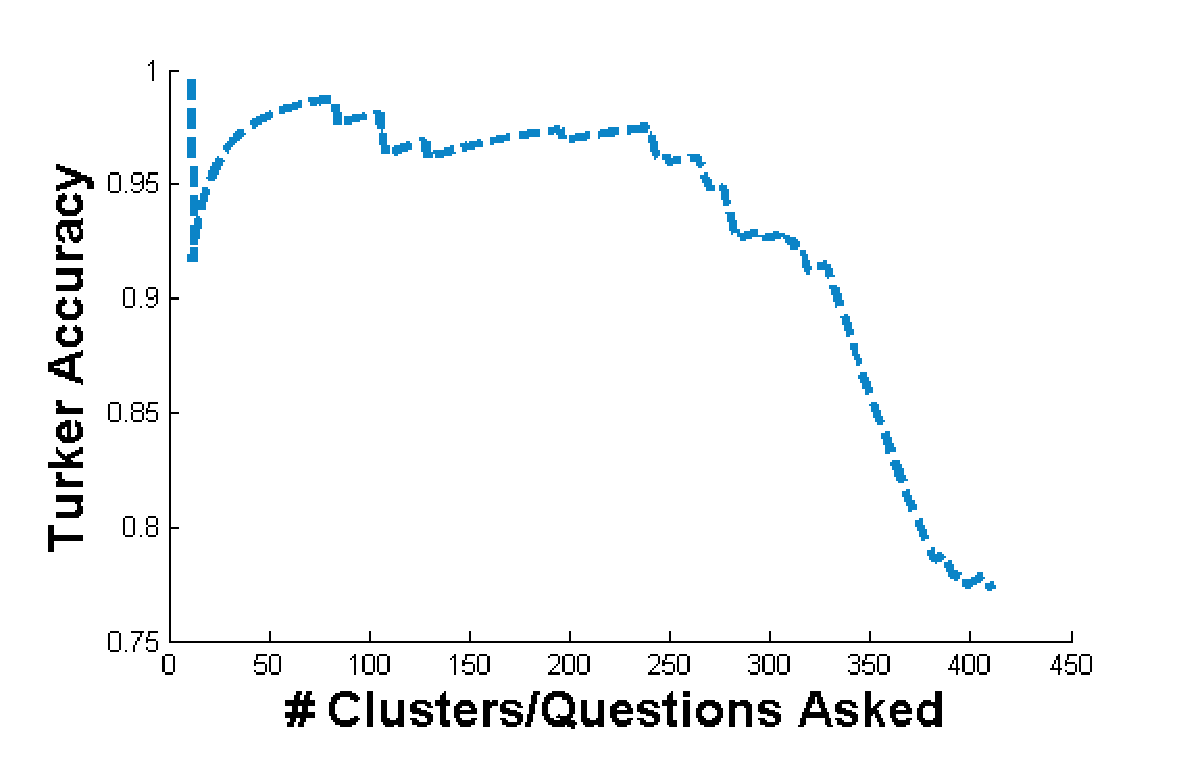
\includegraphics[width=0.95\textwidth]{recall_dblp.eps}
        \caption{Accuracy vs. recall plot for the DBLP-hard data set using probabilistic integration.  If an entropy threshold is set in advance, a high accuracy can be obtained across all accepted answers.}
        \label{fig:recall}
\end{figure}

In addition, one can improve accuracy even further by only accepting those answers for which there is high confidence.  Our probabilistic approach lends itself to a natural confidence indicator in the entropy of the combined distribution.  The trade-off between accuracy and recall is a new functionality compared to deterministic integration which adds flexibility for users to tune the system according to the needs of their application (ie. high accuracy vs. high recall).  Figure~\ref{fig:recall} shows how the accuracy varies for the DBLP-hard set based on how many answers we accept as determined by a confidence threshold.  The initial accuracy was 77\%, but by retaining only the top two-thirds of the answers in this set, we can keep the total accuracy above 90\%.  Previous work~\cite{Sheng:2008:GLI:1401890.1401965} has attempted selectivity by answer entropy.% however, we believe we are the first to probabilistically incorporate Turker reliability into the method.

\eat{
The remaining answers can then be immediately sent back to the crowd for additional querying until their entropy falls below the threshold or a maximum number of answers are received.  This also helps the system identify particularly difficult or troublesome questions.

Originally, we introduced new methods for integration in order to produce a probabilistic result that could provide information on confidence of a crowd combined answer (using its entropy) as well as maintain states of conflict when integrating with additional machine evidence.  What we also find, however, is that we can expect an accuracy boost in addition to new probabilistic features afforded over deterministic integration.  The accuracy gain in the three tables of Figure~\ref{fig:table} compare favorably with the gain observed in Figure~\ref{fig:integrate2}.
}

\noindent\textbf{Summary:} Our experiments show a large savings in cost and gain in accuracy over previous methods.  Selecting those tokens with maximum within-document mutual information and strongest clustering produce an orders-of-magnitude improvement in the number of questions needed compared to random.  Integrating multiple answers probabilistically provides an increase in accuracy by reasoning over Turker uncertainty.  The results in Figure~\ref{fig:table} from real Turker experiments are consistent with those observed synthetically in Figure~\ref{fig:integrate2}.  Finally, probabilistic integration shows promise in providing users with a trade-off between accuracy and recall.
